% Figure from MATH 591 notes, section 8. Compile with the notes preamble.
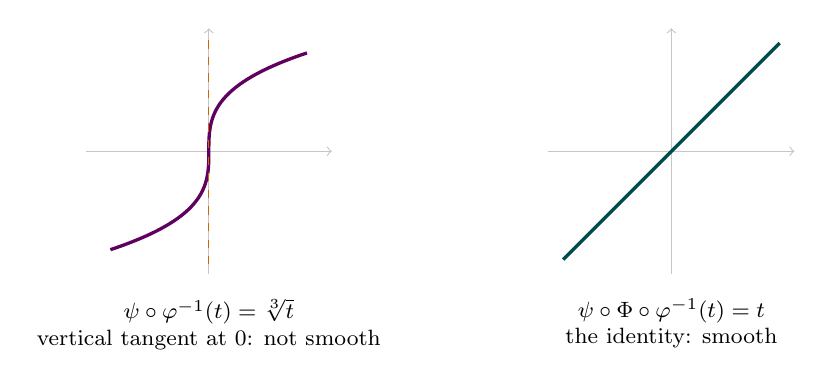
\begin{tikzpicture}[scale=1.25]
\draw[gray!45,->] (-1.25,0)--(1.25,0); \draw[gray!45,->] (0,-1.25)--(0,1.25);
\draw[violet!75!black,very thick,domain=-1:1,samples=90,smooth,variable=\t] plot ({\t*\t*\t},{\t});
\draw[orange!80!black,dashed] (0,-1.15) -- (0,1.15);
\node[font=\footnotesize,align=center,anchor=north] at (0,-1.4) {$\psi\circ\varphi^{-1}(t)=\sqrt[3]{t}$\\ vertical tangent at $0$: not smooth};
\begin{scope}[xshift=4.7cm]
\draw[gray!45,->] (-1.25,0)--(1.25,0); \draw[gray!45,->] (0,-1.25)--(0,1.25);
\draw[teal!60!black,very thick] (-1.1,-1.1) -- (1.1,1.1);
\node[font=\footnotesize,align=center,anchor=north] at (0,-1.4) {$\psi\circ\Phi\circ\varphi^{-1}(t)=t$\\ the identity: smooth};
\end{scope}
\end{tikzpicture}
